\documentclass[a4paper,12pt]{article}
\usepackage[T1]{fontenc}
\usepackage[utf8]{inputenc}
\usepackage{polski}
\usepackage{color}
\usepackage{graphicx}
\usepackage{amsmath}
\usepackage{amssymb}
\usepackage{hyperref}
\usepackage{float}
\usepackage{listings}
\usepackage[backend=biber]{biblatex}

\addbibresource{bibliografia.bib}

\lstset{
  basicstyle=\ttfamily,
  columns=flexible,
  keepspaces=true,
  literate={ą}{{\k{a}}}1
           {ć}{{\'{c}}}1
           {ę}{{\k{e}}}1
           {ł}{{\l{}}}1
           {ń}{{\'{n}}}1
           {ó}{{\'{o}}}1
           {ś}{{\'{s}}}1
           {ź}{{\'{z}}}1
           {ż}{{\.{z}}}1
           {Ą}{{\k{A}}}1
           {Ć}{{\'{C}}}1
           {Ę}{{\k{E}}}1
           {Ł}{{\L{}}}1
           {Ń}{{\'{N}}}1
           {Ó}{{\'{O}}}1
           {Ś}{{\'{S}}}1
           {Ź}{{\'{Z}}}1
           {Ż}{{\.{Z}}}1
}

\title{2. sprawozdanie z laboratorium Hurtownie Danych}
\author{Mikołaj Kubś, 272662}
\date{\today}

\begin{document}

\maketitle

\section{Zadanie 1. Ekstrakcja danych}

\subsection{}

Utworzyć zestawienie, które dla poszczególnych miesięcy i lat przedstawi informację o liczbie różnych klientów. Przygotuj zapytanie z i bez użycia polecenia pivot.

\subsubsection{Wersja bez pivot}

\begin{lstlisting}[
    language=SQL,
    showspaces=false,
    basicstyle=\ttfamily,
    numbers=left,
    numberstyle=\tiny,
    commentstyle=\color{green}
    tabsize=2
    ]
SELECT 
YEAR(OrderDate) AS "Rok", 
MONTH(OrderDate) AS "Miesiąc", 
COUNT(DISTINCT CustomerID) AS "Liczba różnych klientów"
FROM Sales.SalesOrderHeader
GROUP BY YEAR(OrderDate), MONTH(OrderDate)
ORDER BY YEAR(OrderDate), MONTH(OrderDate)
\end{lstlisting}

\begin{figure}[H]
    \centering
    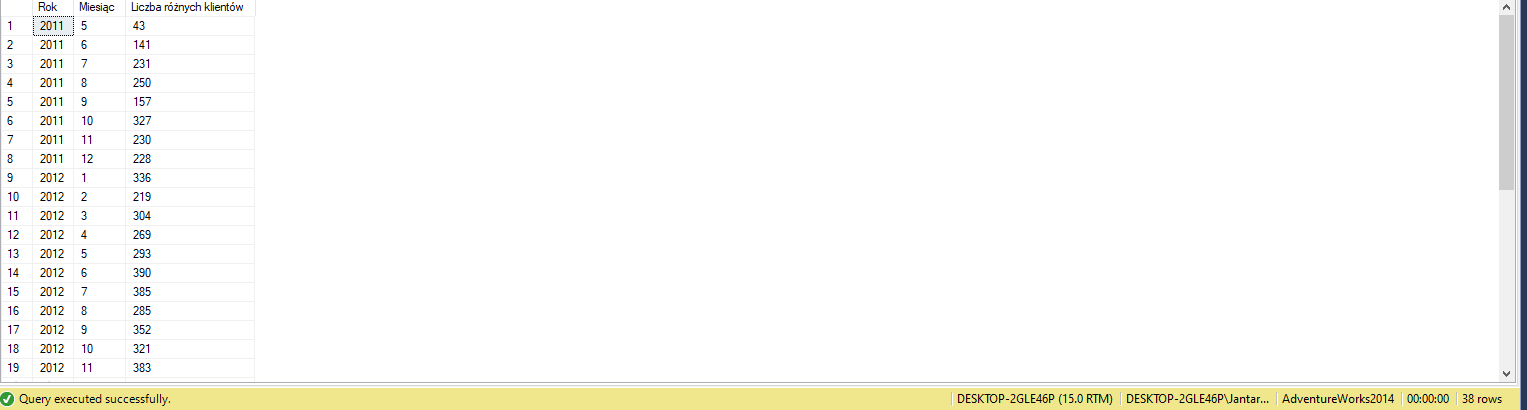
\includegraphics[width=0.8\textwidth]{images/01_normal.png}
    \caption{Wynik wykonania kwerendy 1}
    \label{fig:1_normal}
\end{figure}

\subsubsection{Wersja z użyciem pivot}

\begin{lstlisting}[
    language=SQL,
    showspaces=false,
    basicstyle=\ttfamily,
    numbers=left,
    numberstyle=\tiny,
    commentstyle=\color{green},
    tabsize=2
    ]
WITH UniqueCustomers AS (
    SELECT 
        YEAR(OrderDate) AS OrderYear, 
        MONTH(OrderDate) AS OrderMonth, 
        CustomerID
    FROM Sales.SalesOrderHeader
    GROUP BY YEAR(OrderDate), MONTH(OrderDate), CustomerID
)
SELECT * FROM UniqueCustomers
PIVOT (
    COUNT(CustomerID) 
    FOR OrderMonth IN ([1], [2], [3], [4], 
                       [5], [6], [7], [8], 
                       [9], [10], [11], [12])
) AS PivotTable
ORDER BY OrderYear;
\end{lstlisting}

\begin{figure}[H]
    \centering
    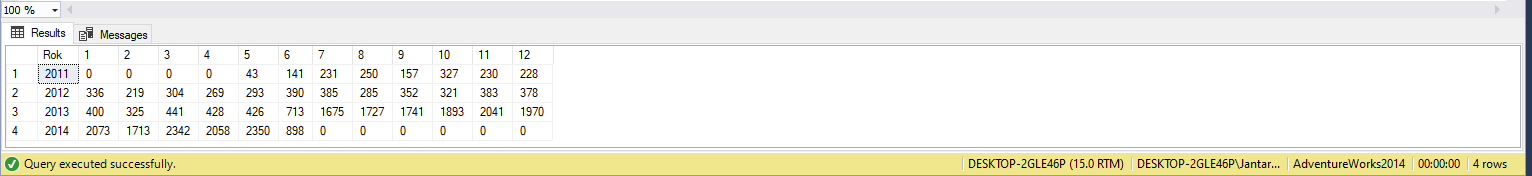
\includegraphics[width=0.8\textwidth]{images/01_pivot.png}
    \caption{Wynik wykonania kwerendy 1 z pivot}
    \label{fig:1_pivot}
\end{figure}

\subsection{}

Utworzyć zestawienie zawierające w wierszach imiona i nazwiska sprzedawców, a w kolumnach kolejne lata. Wartością będzie liczba obsłużonych transakcji. Wyświetlić tylko tych sprzedawców, którzy pracowali przez wszystkie 4 lata.

\begin{lstlisting}[
    language=SQL,
    showspaces=false,
    basicstyle=\ttfamily,
    numbers=left,
    numberstyle=\tiny,
    commentstyle=\color{green},
    tabsize=2
    ]
SELECT * FROM
(
	SELECT 
        FirstName, LastName, SalesOrderID, 
        YEAR(OrderDate) AS OrderYear FROM Sales.SalesPerson
	JOIN HumanResources.Employee ON 
        Employee.BusinessEntityID = SalesPerson.BusinessEntityID
	JOIN Person.Person ON 
        Person.BusinessEntityID = Employee.BusinessEntityID
	JOIN Sales.SalesOrderHeader ON 
        SalesOrderHeader.SalesPersonID = SalesPerson.BusinessEntityID
	WHERE YEAR(HireDate) = 2011
) AS SourceTable
PIVOT (
	COUNT(SalesOrderID)
	FOR OrderYear IN ([2011], [2012], [2013], [2014])
) AS PivotedTable
ORDER BY FirstName
\end{lstlisting}

\begin{figure}[H]
    \centering
    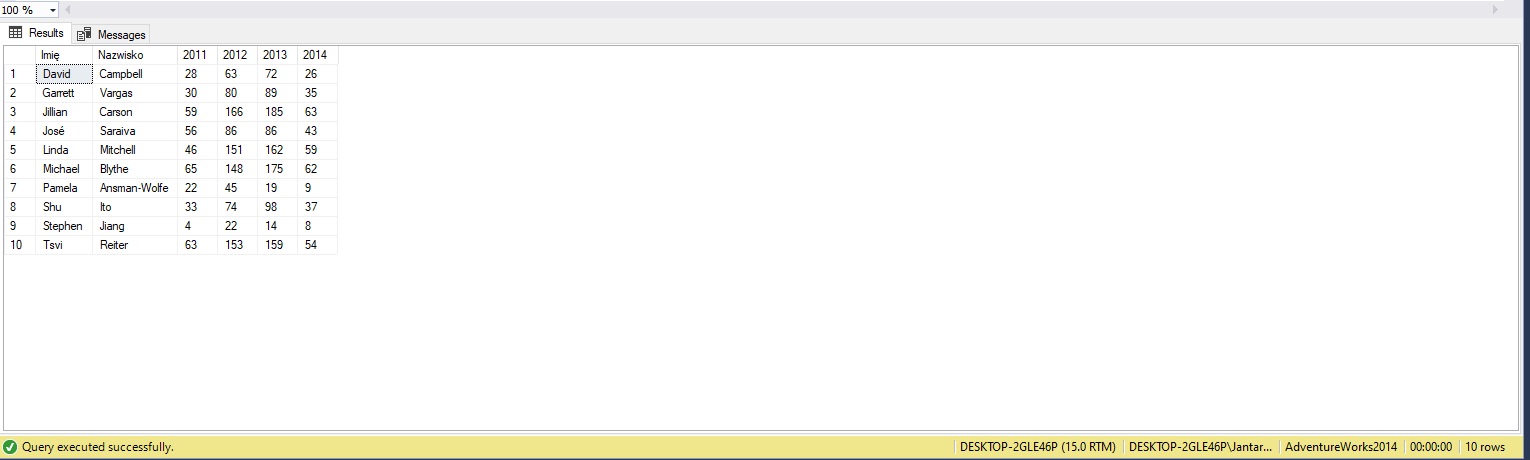
\includegraphics[width=0.8\textwidth]{images/02.png}
    \caption{Wynik wykonania kwerendy 2}
\end{figure}

\subsection{}

Zdefiniować zapytanie wyznaczające sumę kwot sprzedaży towarów oraz liczbę różnych produktów w zamówieniach w poszczególnych latach, miesiącach, dniach.

\begin{lstlisting}[
    language=SQL,
    showspaces=false,
    basicstyle=\ttfamily,
    numbers=left,
    numberstyle=\tiny,
    commentstyle=\color{green},
    tabsize=2
    ]
SELECT 
    YEAR(OrderDate) AS "Rok", 
    MONTH(OrderDate) AS "Miesiąc", 
    DAY(OrderDate) AS "Dzień", 
    SUM(LineTotal) AS "Suma", 
    COUNT(DISTINCT ProductID) AS "Liczba różnych produktów"
FROM Sales.SalesOrderHeader
JOIN Sales.SalesOrderDetail ON 
    SalesOrderDetail.SalesOrderID = SalesOrderHeader.SalesOrderID
GROUP BY YEAR(OrderDate), MONTH(OrderDate), DAY(OrderDate)
ORDER BY YEAR(OrderDate), MONTH(OrderDate), DAY(OrderDate)
\end{lstlisting}

\begin{figure}[H]
    \centering
    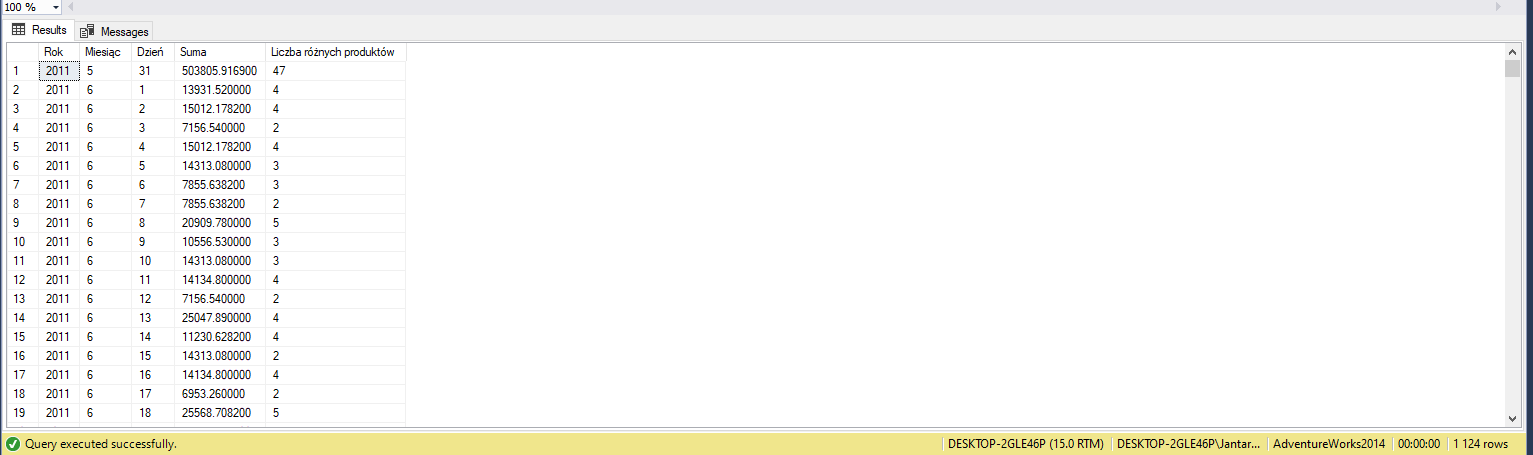
\includegraphics[width=0.8\textwidth]{images/03.png}
    \caption{Wynik wykonania kwerendy 3}
\end{figure}

\subsection{}

Wykorzystując polecenie CASE przygotować podsumowania do zestawienia z poprzedniego zadania tak, aby sumowane były kwoty zamówień oraz obliczana liczba różnych produktów dla poszczególnych miesięcy i dni tygodnia.\\
Uwaga: Pamiętaj o wybraniu właściwego atrybutu funkcji datepart tak, aby zgadzała się nazwa dnia tygodnia

\begin{lstlisting}[
    language=SQL,
    showspaces=false,
    basicstyle=\ttfamily,
    numbers=left,
    numberstyle=\tiny,
    commentstyle=\color{green},
    tabsize=2
    ]
SET DATEFIRST 1;
SET LANGUAGE Polish;

SELECT 
    YEAR(OrderDate) AS "Rok", 
    DATENAME(month, OrderDate) AS "Miesiąc",     
    CASE DATEPART(dw, OrderDate)
        WHEN 1 THEN 'Poniedziałek'
        WHEN 2 THEN 'Wtorek'
        WHEN 3 THEN 'Środa'
        WHEN 4 THEN 'Czwartek'
        WHEN 5 THEN 'Piątek'
        WHEN 6 THEN 'Sobota'
        WHEN 7 THEN 'Niedziela'
    END AS "Dzień tygodnia", 
    SUM(LineTotal) AS "Suma", 
    COUNT(DISTINCT ProductID) AS "Liczba różnych produktów"
FROM Sales.SalesOrderHeader
JOIN Sales.SalesOrderDetail ON 
    SalesOrderDetail.SalesOrderID = SalesOrderHeader.SalesOrderID
GROUP BY 
    YEAR(OrderDate), 
    DATENAME(month, OrderDate),
    MONTH(OrderDate),
    DATEPART(dw, OrderDate)
ORDER BY 
    YEAR(OrderDate), 
    MONTH(OrderDate), 
    DATEPART(dw, OrderDate)
\end{lstlisting}

\begin{figure}[H]
    \centering
    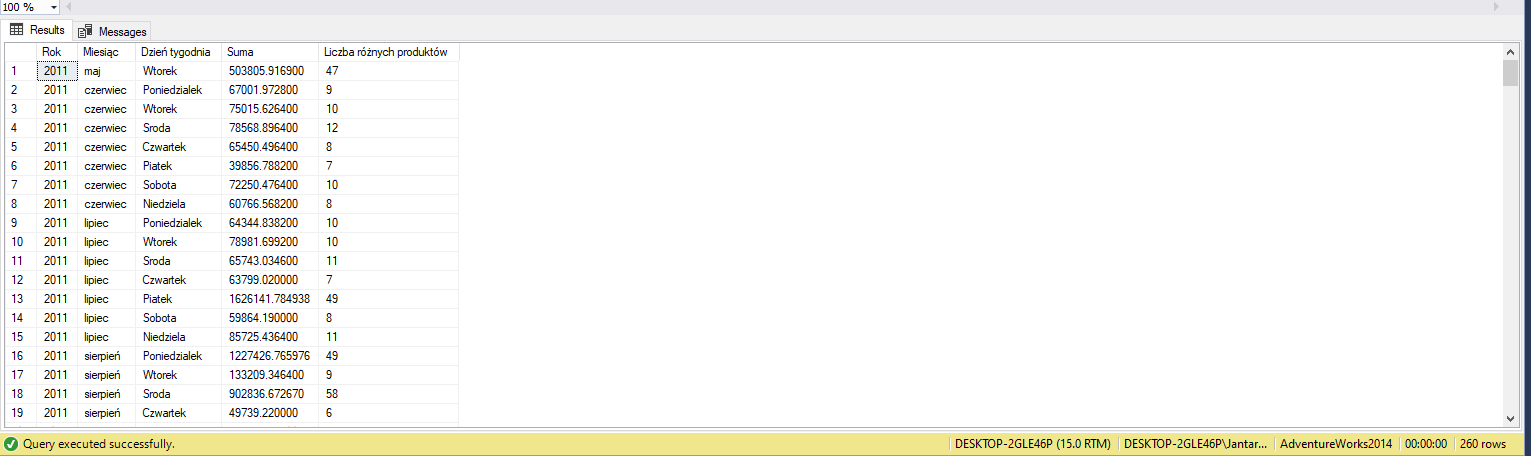
\includegraphics[width=0.8\textwidth]{images/04.png}
    \caption{Wynik wykonania kwerendy 4}
\end{figure}

\subsection{}

Przygotować zestawienie, w którym dla wybranych klientów przygotujemy kartę lojalnościową:\\
a. srebrną, jeśli klient wykonał co najmniej 2 transakcje w sklepie;\\
b. złotą, jeśli wykonał co najmniej 4 transakcje w sklepie, w tym co najmniej 2 transakcje, których łączna kwota przekraczała 250\% średniej wartości zamówień w bazie;\\
c. platynową, jeśli klient spełniał warunki otrzymania karty złotej oraz w co najmniej jednej transakcji kupił jednocześnie produkty ze wszystkich kategorii

\begin{lstlisting}[
    language=SQL,
    showspaces=false,
    basicstyle=\ttfamily,
    numbers=left,
    numberstyle=\tiny,
    commentstyle=\color{green},
    tabsize=2
    ]
WITH AvgOrderValue AS (
    SELECT AVG(TotalOrderValue) AS AvgValue
    FROM (
        SELECT SalesOrderID, SUM(LineTotal) AS TotalOrderValue
        FROM Sales.SalesOrderDetail
        GROUP BY SalesOrderID
    ) AS OrderValues
),
OrderCount AS (
    SELECT CustomerID, COUNT(DISTINCT SalesOrderID) AS TransactionCount,
            SUM(TotalDue) AS TotalTransactionValue
    FROM Sales.SalesOrderHeader
    GROUP BY CustomerID
),
HighValueOrders AS (
    SELECT CustomerID, COUNT(*) AS HighValueOrderCount
    FROM (
        SELECT SalesOrderID, SUM(LineTotal) AS TotalOrderValue
        FROM Sales.SalesOrderDetail
        GROUP BY SalesOrderID
    ) AS OrderValues
    JOIN Sales.SalesOrderHeader 
        ON SalesOrderHeader.SalesOrderID = OrderValues.SalesOrderID
    CROSS JOIN AvgOrderValue A 
    WHERE TotalOrderValue > 2.5 * A.AvgValue
    GROUP BY CustomerID
),
UniqueCategories AS (
    SELECT 
        C.CustomerID, 
        COUNT(DISTINCT PC.ProductCategoryID) AS UniqueCategories
    FROM Sales.Customer C
    JOIN Sales.SalesOrderHeader SOH 
        ON SOH.CustomerID = C.CustomerID
    JOIN Sales.SalesOrderDetail SOD 
        ON SOD.SalesOrderID = SOH.SalesOrderID
    JOIN Production.Product PR ON PR.ProductID = SOD.ProductID
    JOIN Production.ProductSubcategory PSC 
        ON PSC.ProductSubcategoryID = PR.ProductSubcategoryID
    JOIN Production.ProductCategory PC 
        ON PC.ProductCategoryID = PSC.ProductCategoryID
    GROUP BY C.CustomerID
)
SELECT 
    P.FirstName AS Imie, 
    P.LastName AS Nazwisko, 
    COALESCE(OrderCount.TransactionCount, 0) AS "Liczba transakcji",
    COALESCE(OrderCount.TotalTransactionValue, 0) AS "Łączna kwota transakcji",
    CASE 
        WHEN COALESCE(OrderCount.TransactionCount, 0) >= 4 
            AND COALESCE(HighValueOrders.HighValueOrderCount, 0) >= 2 
            AND COALESCE(UniqueCategories.UniqueCategories, 0) = 
            (SELECT COUNT(*) FROM Production.ProductCategory) 
            THEN 'Platynowa'
        WHEN COALESCE(OrderCount.TransactionCount, 0) >= 4 
            AND COALESCE(HighValueOrders.HighValueOrderCount, 0) >= 2 
            THEN 'Złota'
        WHEN COALESCE(OrderCount.TransactionCount, 0) >= 2 
            THEN 'Srebrna'
        ELSE 'Brak karty'
    END AS "Kolor karty"
FROM Sales.Customer C
JOIN Person.Person P ON P.BusinessEntityID = C.PersonID
LEFT JOIN HighValueOrders ON HighValueOrders.CustomerID = C.CustomerID
LEFT JOIN OrderCount ON OrderCount.CustomerID = C.CustomerID
LEFT JOIN UniqueCategories ON UniqueCategories.CustomerID = C.CustomerID
ORDER BY OrderCount.TotalTransactionValue DESC;    
\end{lstlisting}

\begin{figure}[H]
    \centering
    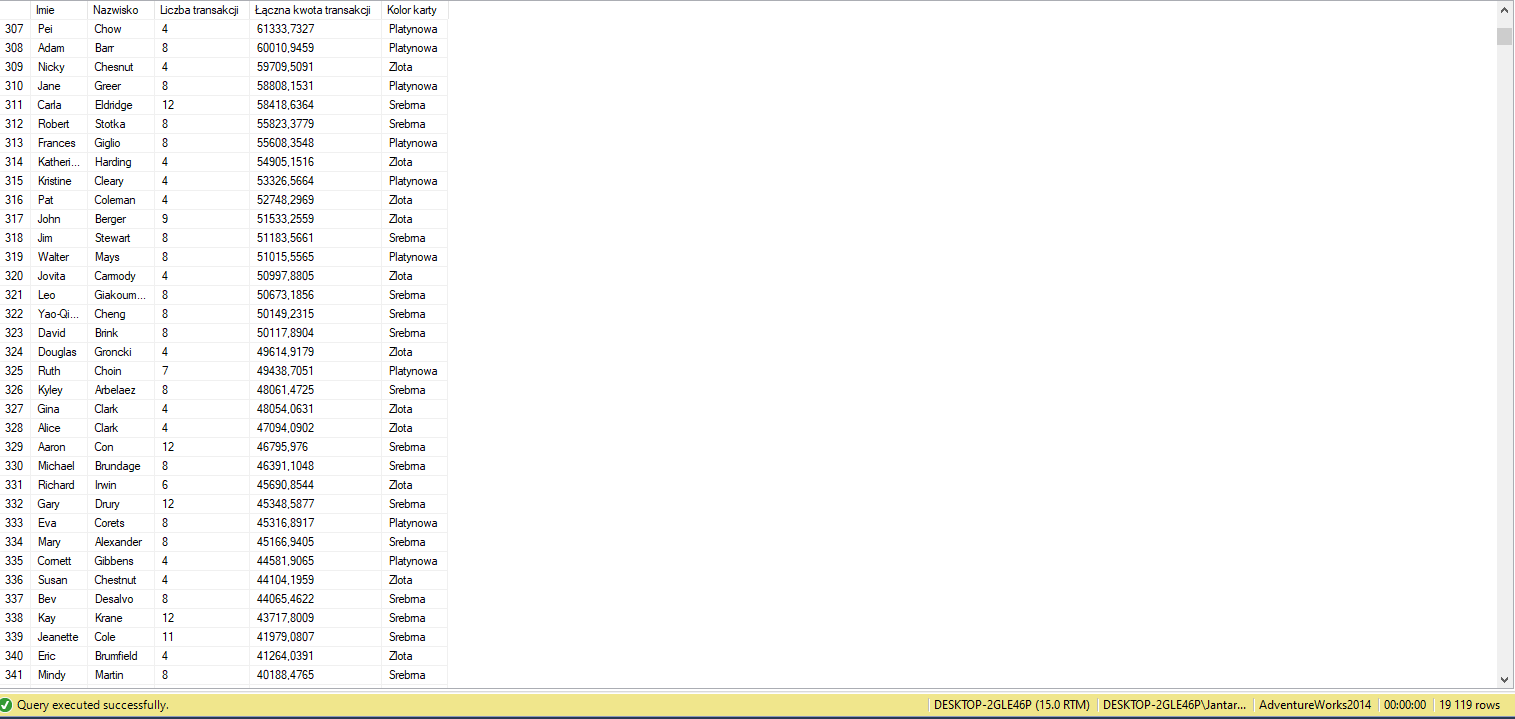
\includegraphics[width=0.8\textwidth]{images/05.png}
    \caption{Wynik wykonania kwerendy 5}
\end{figure}

\section{Zadanie 2. Analiza danych}

\subsection{}

Przedstaw wyniki zadania 1 w postaci tabel i wykresów przestawnych w programie MS Excel. Zinterpretuj wyniki.

\subsubsection{}

\begin{figure}[H]
    \centering
    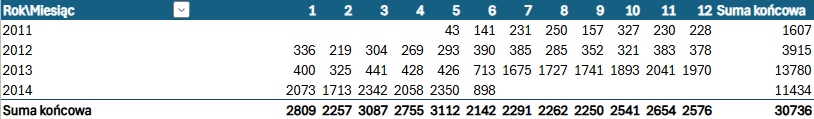
\includegraphics[width=0.8\textwidth]{images/excel/01.png}
    \caption{Tabela przestawna na podstawie wyników kwerendy 1}
\end{figure}

Można zauważyć stabilny trend wzrostowy w liczbie klientów wraz z czasem. W lipcu 2013 roku do firmy przybyło aż prawie 900 klientów, co było zdecydowanie największym wzrostem. Kolejną anomalią jest lipiec 2014 roku. Mimo posiadania danych z całego miesiąca, liczba różnych klientów zmniejszyła się ponad dwukrotnie i osiągnęła najniższy poziom od czerwca 2013 roku. Dane za cały miesiąc były niskie. Nie było też żadnego dnia, w którym sklep miał ponad dwukrotność średniej klientów na miesiąc, jak to bywało w innych miesiącach.

\subsubsection{}

\begin{figure}[H]
    \centering
    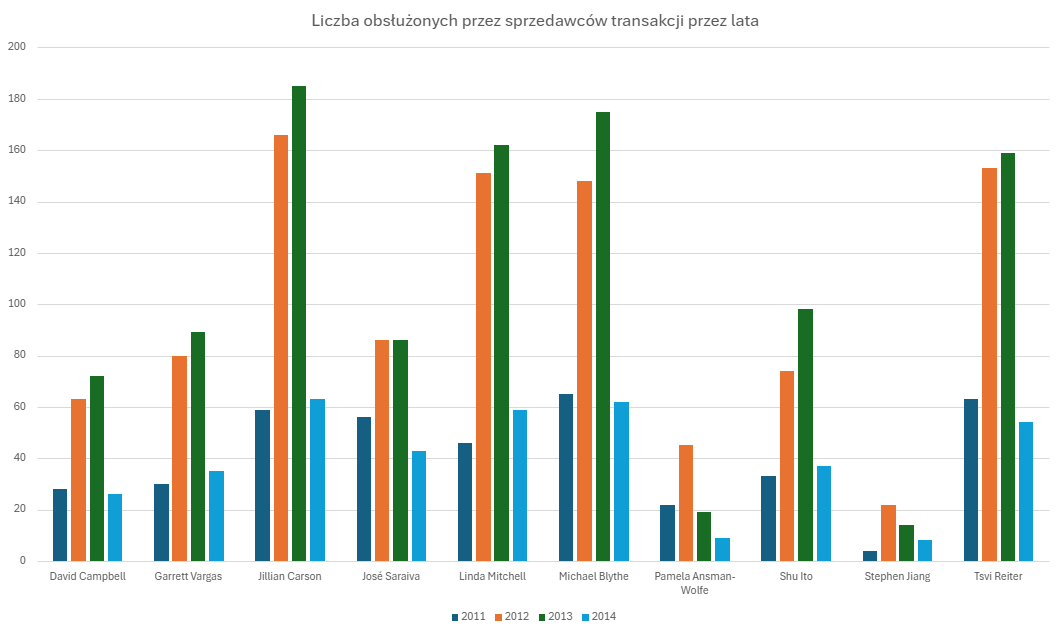
\includegraphics[width=0.8\textwidth]{images/excel/02.png}
    \caption{Wykres na podstawie wyników kwerendy 2}
\end{figure}

Różnice między liczbą obsłużonych klientów między sprzedawcami są bardzo duże. Jest 4 sprzedawców, którzy pozytywnie wyróżniają się na tle reszty, i dwóch sprzedawców w odwrotnej sytuacji. Na tym wykresie również można zauważyć potwierdzony w innych kwerendach trend wzrostowy sklepu w liczbie klientów. Jak widać na wykresie, dla prawie każdego sprzedawcy liczba obsłużonych klientów w 2012 lub 2013 jest znacznie wyższa niż w 2011. 2014 jeszcze się nie skończył i jest nadzieja na dobry sezon wakacyjny, dzięki któremu poziom poprzednich 2 lat może być utrzymany. 

\subsubsection{}

\begin{figure}[H]
    \centering
    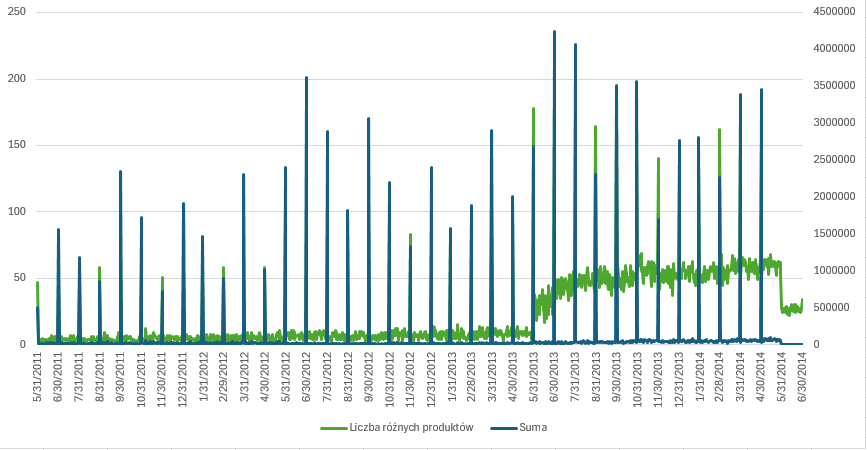
\includegraphics[width=0.8\textwidth]{images/excel/03.png}
    \caption{Wykres na podstawie wyników kwerendy 3}
\end{figure}

Od razu zauważalna jest pewna niespójność w danych - mniej więcej co miesiąc (na samym początku lub końcu miesiąca) liczba sprzedanych różnych produktów i suma sprzedaży osiągają wielokrotność wyników w innych dniach. Poza tym widać trend wzrostowy, wraz z nagłym silnym wzrostem sprzedaży, który został zauważony w poprzednich analizach. Tak jak w poprzednich analizach, ostatni miesiąc ma o około połowę niższą sprzedaż niż poprzednie.

\subsubsection{}

\begin{figure}[H]
    \centering
    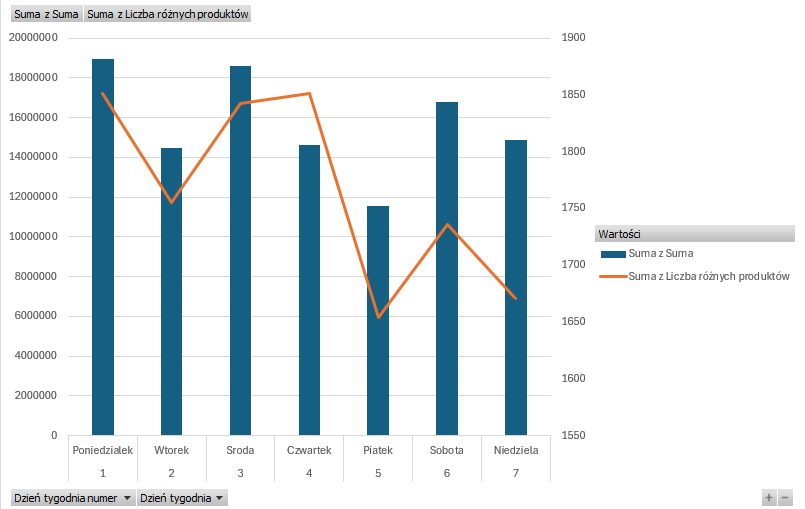
\includegraphics[width=0.8\textwidth]{images/excel/04.png}
    \caption{Wykresy na podstawie wyników kwerendy 4}
\end{figure}

Wykres pokazuje, że nie ma bezpośredniej korelacji między liczbą różnych produktów a sumą sprzedaży. Na przykład niedziela charakteryzuje się podobną liczbą różnych produktów co piątek, ale wyraźnie wyższą wartością sprzedaży.

Piątek wyróżnia się najniższą liczbą produktów i najniższą sprzedażą, podczas gdy poniedziałek i środa osiągają najwyższe wartości. W weekend sobota generuje wyższe przychody i większą liczbę sprzedanych produktów niż niedziela.

\subsubsection{}

\begin{figure}[H]
    \centering
    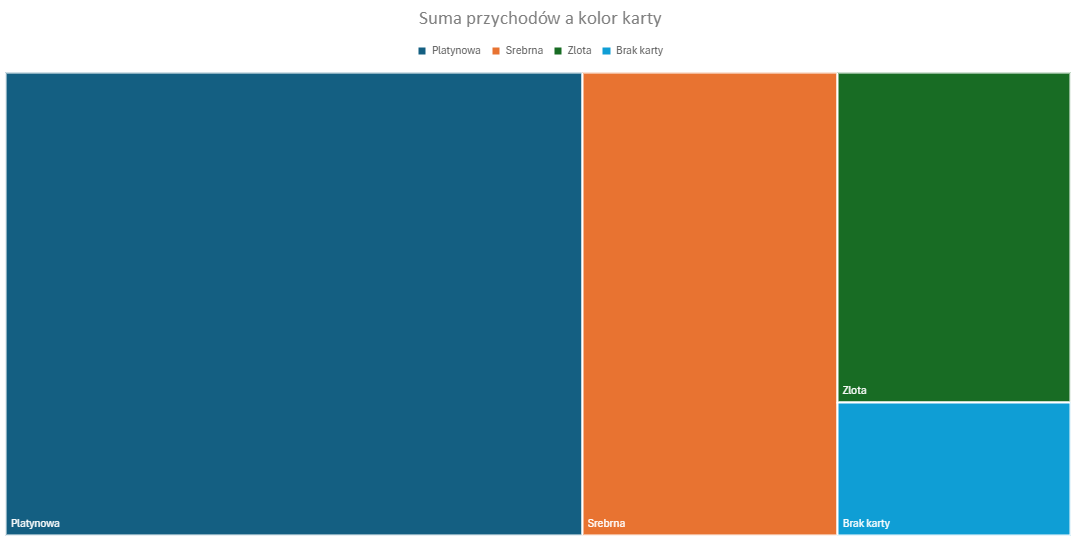
\includegraphics[width=0.8\textwidth]{images/excel/05.png}
    \caption{Wykres na podstawie wyników kwerendy 5}
\end{figure}

Z wykresu drzewa można wyczytać, że największa suma wartości przypada na karty platynowe, które zajmują największą powierzchnię na wykresie. Karty srebrne są drugie pod względem sumy, natomiast karty złote i brak karty mają mniejsze wartości, przy czym "brak karty" ma najmniejszy udział. Wykres ten dobrze obrazuje proporcje między kategoriami, pokazując, że platynowe karty mają zdecydowaną dominację. Z tego wynika, że za większość obrotów sklepu odpowiadają stali klienci. Kupili oni coś przynajmniej 4 razy, przynajmniej raz bardzo różnorodne zakupy i przynajmniej 2 razy zakupy o wartości znacznie przewyższającej średnią. Złota karta odpowiada za stan przejściowy między srebrną a platynową, co sugeruje możliwość zmiany wielu klientów w tych najbardziej dochodowych.

\subsection{}

Przygotuj 5 dodatkowych tabel/wykresów, które pokażą ciekawe zależności w bazie AdventureWorks przy użyciu Power BI lub Tableau. Przedstaw wnioski biznesowe wynikające z tych zestawień

\begin{figure}[H]
    \centering
    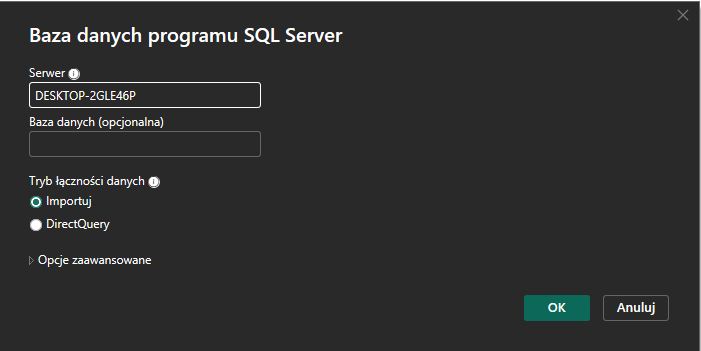
\includegraphics[width=0.8\textwidth]{images/power_bi/connection.png}
    \caption{Połączenie z Power BI}
\end{figure}

\subsubsection{}

\begin{figure}[H]
    \centering
    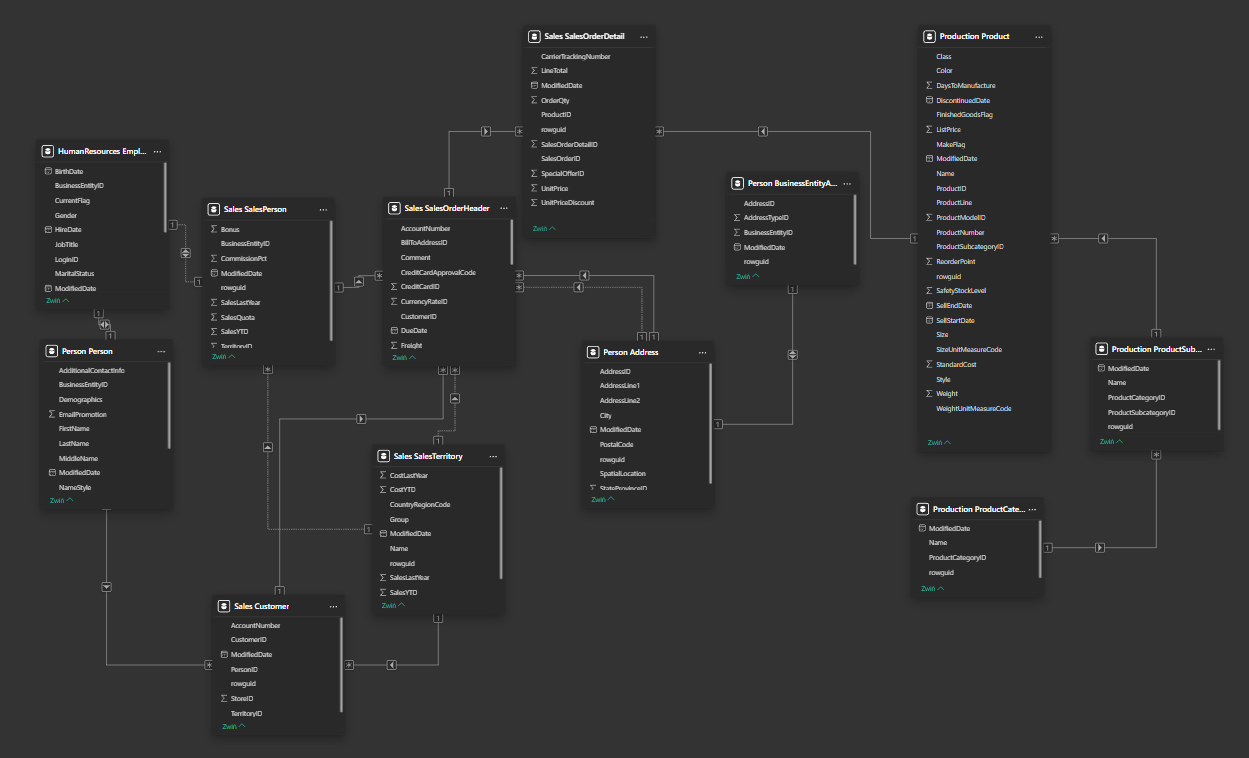
\includegraphics[width=0.8\textwidth]{images/power_bi/model.png}
    \caption{Model danych w Power BI}
\end{figure}

Na wykresie jasno widać, w których państwach sprzedawane są artykuły sklepu. Dodatkowo można porównać wielkości wykresów kołowych, aby zobaczyć wysokość sprzedaży z poprzedniego roku. Wykres kołowy w USA jest podzielony dodatkowo na 5 terytorii, typu Northeast, Southeast itd. Jak łatwo można zauważyć, największa suma sprzedaży jest w Stanach Zjednoczonych i Kanadzie, a najmniejsza w Niemczech.

\subsubsection{}

\begin{figure}[H]
    \centering
    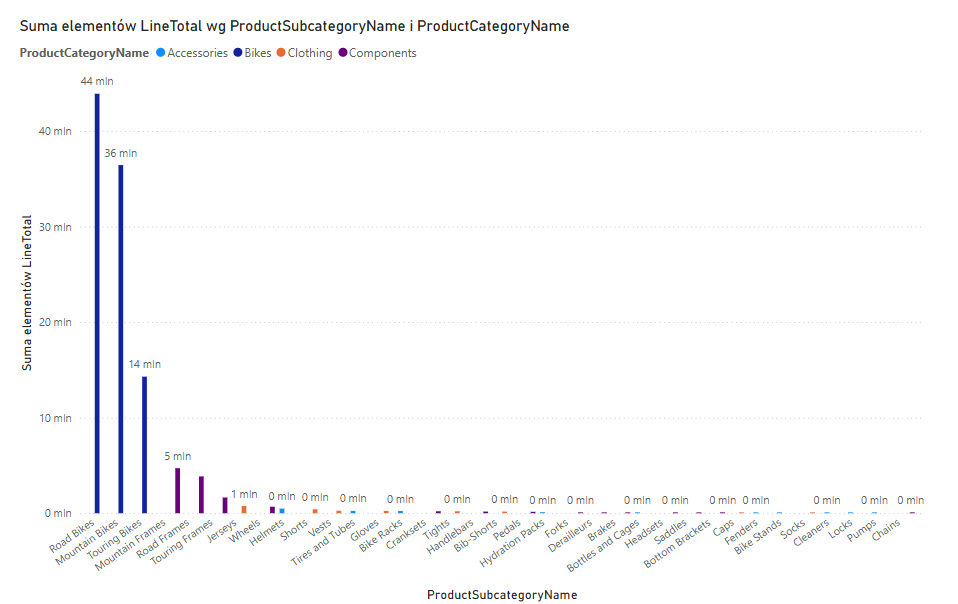
\includegraphics[width=0.8\textwidth]{images/power_bi/02.png}
    \caption{2. wykres w Power BI}
\end{figure}

Sklep uzyskiwał największą sumę przychodów ze sprzedaży różnego rodzaju rowerów. Następne są różne komponenty, ale przychody z nich były znacznie mniejsze. Dzięki temu wykresowi jasno widać, z czego sklep historycznie czerpał jaką część przychodów.

\subsubsection{}

\begin{figure}[H]
    \centering
    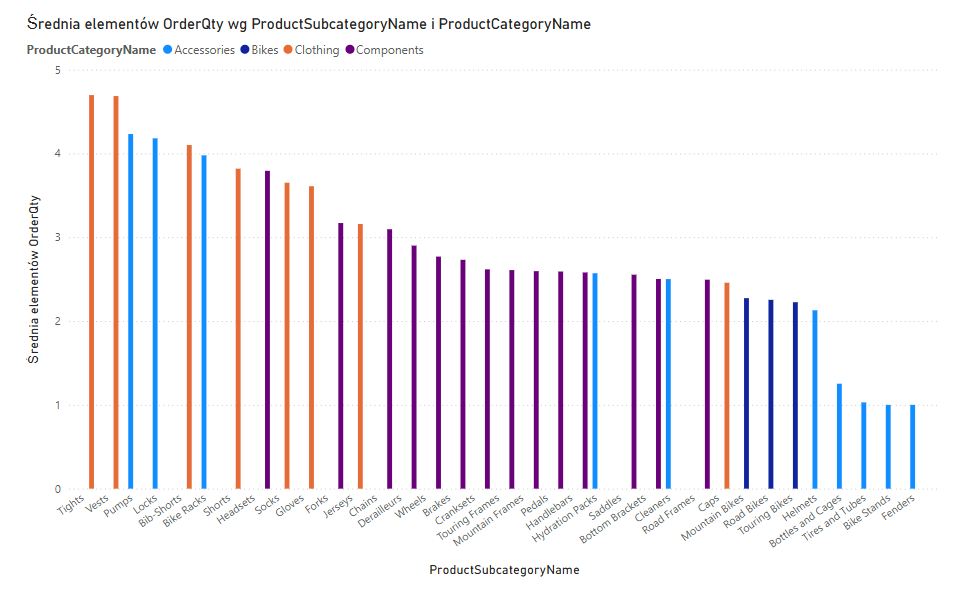
\includegraphics[width=0.8\textwidth]{images/power_bi/03.png}
    \caption{3. wykres w Power BI}
\end{figure}

Na tym wykresie można zauważyć ciekawe zależności. Mimo, iż sklep większość przychodów uzyskuje ze sprzedaży rowerów, średnia liczba kupionych tych samych rowerów nie jest najwyższa. Jak widać na wykresie, dla danego produktu w danej transakcji klienci kupują średnio najwięcej elementów ubioru lub akcesorii, takich jak rajstopy, kamizelki czy pompki. Być może można by ustalić kandydatów na oferty z obniżoną ceną przy wielosztukowaniu na podstawie tego wykresu.

\subsubsection{}

\begin{figure}[H]
    \centering
    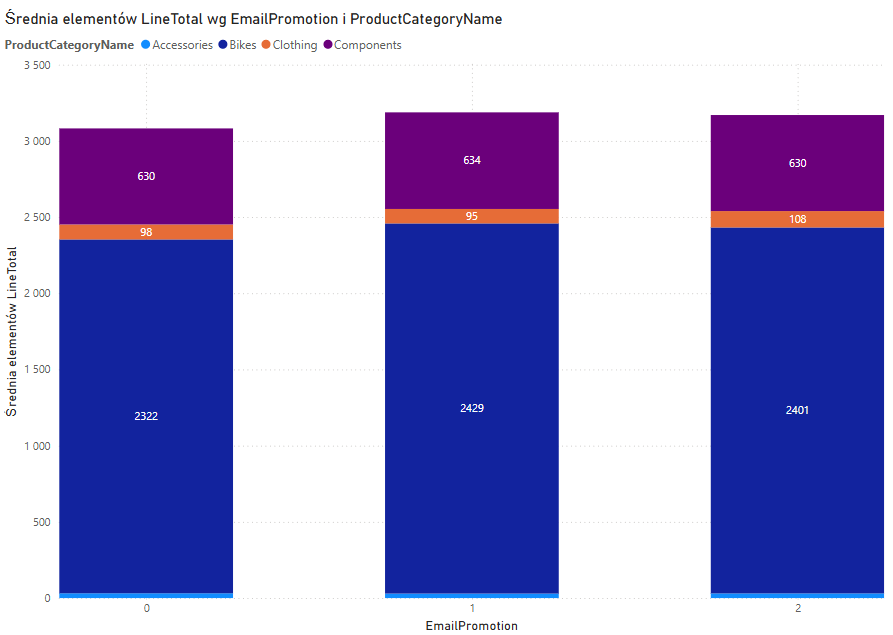
\includegraphics[width=0.8\textwidth]{images/power_bi/04.png}
    \caption{4. wykres w Power BI}
\end{figure}

Według strony dataedo.com \cite{adventureworks} EmailPromotion oznacza:

"0 = Contact does not wish to receive e-mail promotions, 1 = Contact does wish to receive e-mail promotions from AdventureWorks, 2 = Contact does wish to receive e-mail promotions from AdventureWorks and selected partners."

Brakuje korelacji między EmailPromotion a średnią sprzedażą dla danego klienta, co sugeruje, że promocje e-mail nie są specjalnie efektywne. 

\subsubsection{}

\begin{figure}[H]
    \centering
    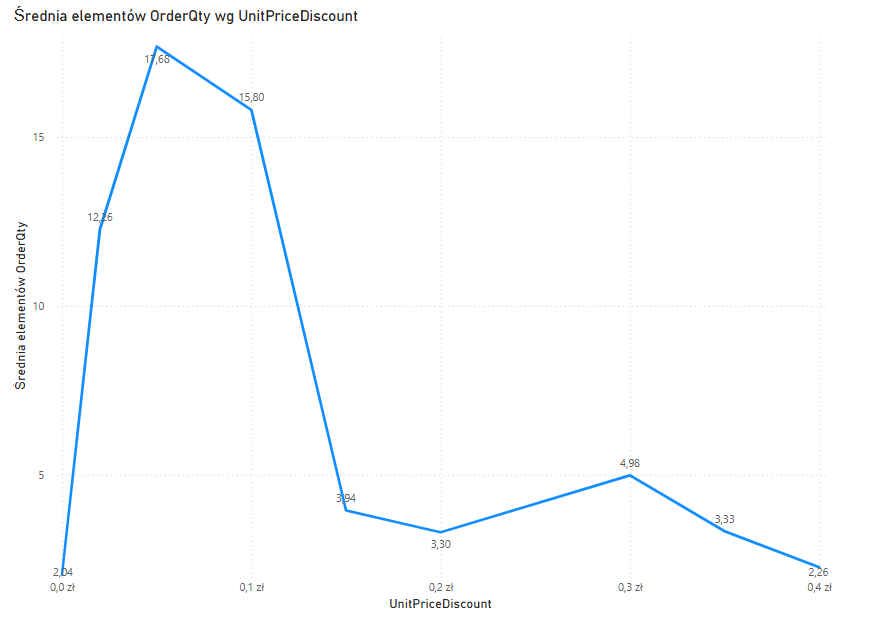
\includegraphics[width=0.8\textwidth]{images/power_bi/05.png}
    \caption{5. wykres w Power BI}
\end{figure}

Brakuje zależności między średnią liczbą zamówionego produktu, a rabatem na niego przeznaczonym. Wykres co prawda na początku rośnie, ale potem szybko spada. Ostatecznie średnia liczba zamówionego produktu jest bardzo podobna dla zerowego rabatu, jak i dla maksymalnego rabatu. Być może wysokie rabaty mają klauzulę ograniczającą, na ile maksymalnie produktów jest rabat.

\section{Wnioski}

Na podstawie przeprowadzonych analiz można sformułować następujące wnioski:

\begin{enumerate}
    \item \textbf{Trend wzrostowy i sezonowość:}  
    Analiza danych wykazała stabilny trend wzrostowy w liczbie klientów, co potwierdzają zarówno wyniki kwerendy 1, jak i wizualizacje w MS Excel. Szczególnie zauważalny jest gwałtowny wzrost w lipcu 2013 roku oraz wyraźna anomalia w lipcu 2014 - miesiącu, w którym liczba klientów spadła znacząco. Może to sugerować wystąpienie czynników sezonowych lub operacyjnych, które warto zbadać w dalszych analizach.

    \item \textbf{Różnice w efektywności sprzedaży:}  
    Zestawienie sprzedażowe według sprzedawców (kwerenda 2) ujawnia duże zróżnicowanie wyników. Kilku sprzedawców wyróżnia się bardzo dobrymi rezultatami, podczas gdy inni osiągają znacznie niższe wyniki. Wskazuje to na potrzebę dalszej analizy efektywności poszczególnych pracowników oraz rozważenie wdrożenia szkoleń, aby wyrównać wyniki zespołu, zmiany pracowników lub dalszej analizy przyczyn.

    \item \textbf{Zależności między ofertą a sprzedażą:}
    Wyniki kwerend 3 i 4 pokazały, że między liczbą różnych produktów a sumą sprzedaży nie występuje bezpośrednia korelacja. Analiza według dni tygodnia wskazuje, że poszczególne dni charakteryzują się odmienną intensywnością sprzedaży - najwyższe wartości odnotowano w poniedziałki i środy, a najniższe w piątki. Może to stanowić podstawę do optymalizacji harmonogramu promocji i działań marketingowych.

    \item \textbf{Znaczenie lojalności klientów:}
    Przygotowana karta lojalnościowa (kwerenda 5) umożliwia segmentację klientów na podstawie liczby transakcji, wartości zakupów oraz różnorodności kategorii produktów. Wyniki wskazują, że klienci z platynowymi kartami generują największy obrót, co podkreśla wagę budowania długoterminowych relacji z klientami. Segmentacja ta może posłużyć do opracowania dalszych programów lojalnościowych.

    \item \textbf{Wnioski z analiz w Power BI:}  
    \begin{itemize}
        \item \textbf{Geograficzna dystrybucja sprzedaży:}
        Wizualizacja danych geograficznych pokazuje, że największe obroty generowane są w USA i Kanadzie, co może wpłynąć na decyzje dotyczące ekspansji rynkowej lub skoncentrowania działań marketingowych w tych regionach.
        
        \item \textbf{Struktura sprzedaży produktów:}
        Największe przychody pochodzą z kategorii rowerów, jednak analiza ilościowa zakupów wskazuje, że produkty ubieralne i akcesoria kupowane są w większych ilościach. Otwiera to możliwości wprowadzenia ofert promocyjnych przy zakupach wieloelementowych.
        
        \item \textbf{Skuteczność promocji e-mailowych:}  
        Brak wyraźnej korelacji między ustawieniem opcji \texttt{EmailPromotion} a średnią sprzedażą sugeruje, że obecne kampanie e-mailowe mogą wymagać rewizji lub lepszego targetowania.
        
        \item \textbf{Strategia rabatowa:}  
        Analiza zależności między średnią ilością zamówionych produktów a przyznawanym rabatem wskazuje, że rabaty nie wpływają znacząco na wielkość zamówień, co może sugerować potrzebę modyfikacji polityki rabatowej lub wprowadzenia dodatkowych ograniczeń.
    \end{itemize}
\end{enumerate}

Podsumowując, przedstawione rozwiązania umożliwiły dogłębną analizę danych sprzedażowych oraz identyfikację kluczowych czynników wpływających na wyniki firmy. Wnioski te mogą stanowić solidną podstawę do podejmowania decyzji biznesowych, optymalizacji strategii sprzedażowych oraz doskonalenia działań marketingowych.

\printbibliography

\end{document}